\subsection{Simulation}

We have simulated the system with $\chi_c = 1 \deg, 5 \deg$ and $10 \deg.$ And with a $\pm 25 \deg$ constraint on $\delta_a$. We obtained the results in figures \ref{fig:2e_1}, \ref{fig:2e_5} and \ref{fig:2e_10}. 
We can see that the system reaches the desired state in approximately a 100 seconds for each simulation, with the last one being the slowest. This makes sense as the desired value is larger and the constraint on $\delta_a$ limits our ability to approach the value faster. In addition, note that this aircraft is probably not a very comfortable ride.

There are a lot of oscillations in the step response of the course. This is because we have simplified the aircraft model and the assumptions aline with the roll mode. In addition the damping frequency $\zeta_\chi$ is set to 1. Had we chosen a larger $\zeta_\chi$ the oscillations would be smaller, due to more damping, but the system would be even slower than it is now. The system is quite slow in attaining the desired state.


\begin{figure}[h!]
    \centering
    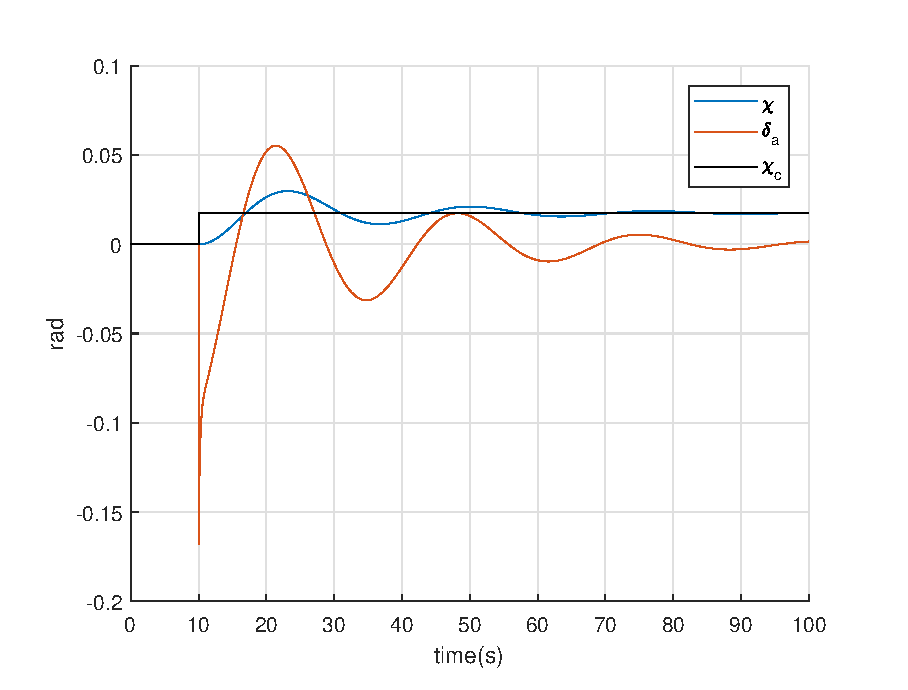
\includegraphics[scale = 0.8]{plots/2e_1.eps}
    \caption{Simulation with a step size of $1 \deg$.}
    \label{fig:2e_1}
\end{figure}

\begin{figure}[h!]
    \centering
    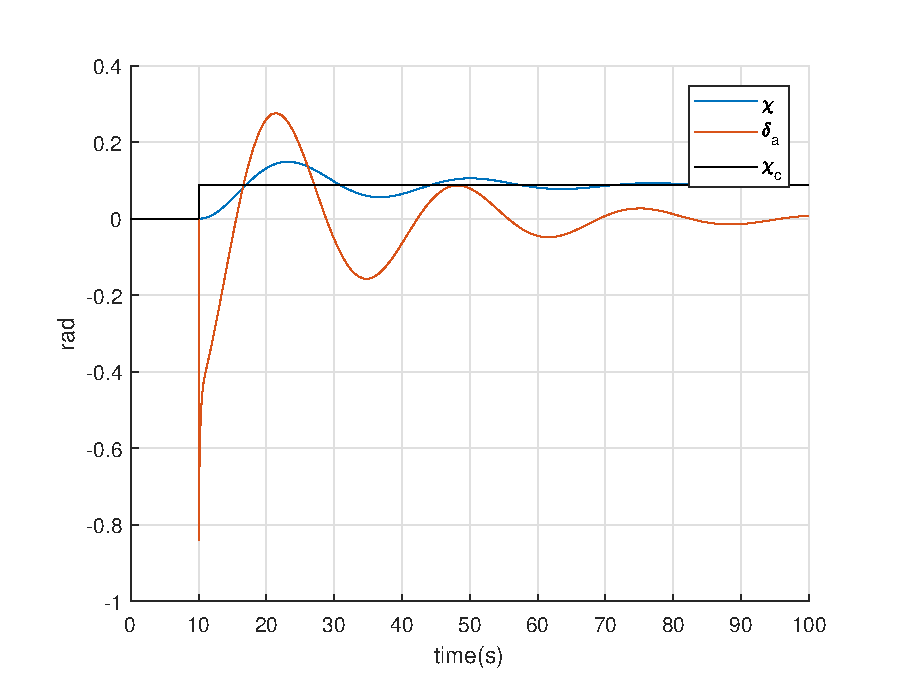
\includegraphics[scale = 0.8]{plots/2e_5.eps}
    \caption{Simulation with a step size of $5 \deg$.}
    \label{fig:2e_5}
\end{figure}

\begin{figure}[h!]
    \centering
    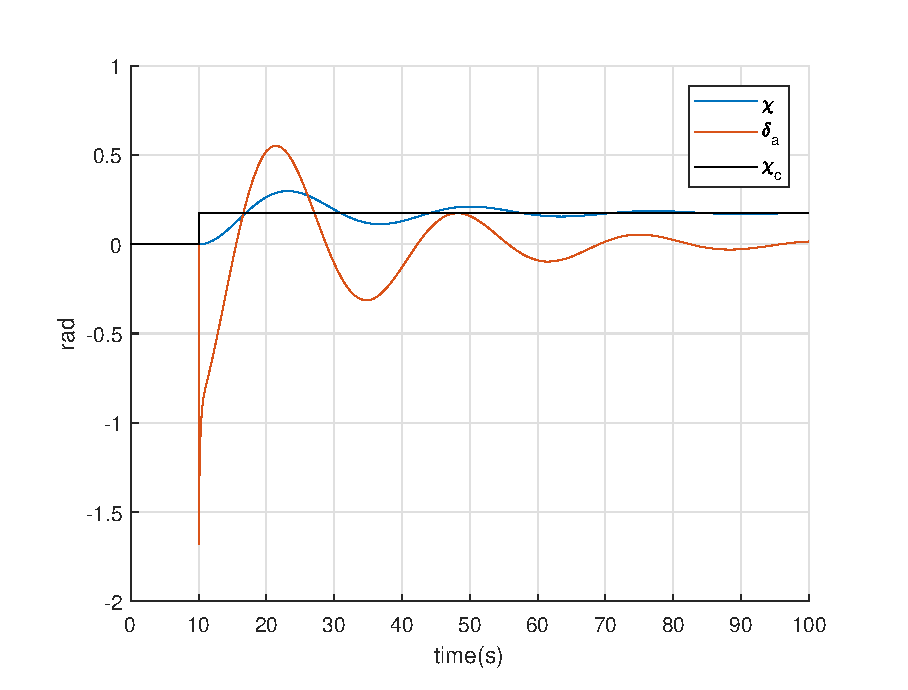
\includegraphics[scale = 0.8]{plots/2e_10.eps}
    \caption{Simulation with a step size of $10 \deg$.}
    \label{fig:2e_10}
\end{figure}

